\chapter{Diskussion}

\begin{figure}[ht]
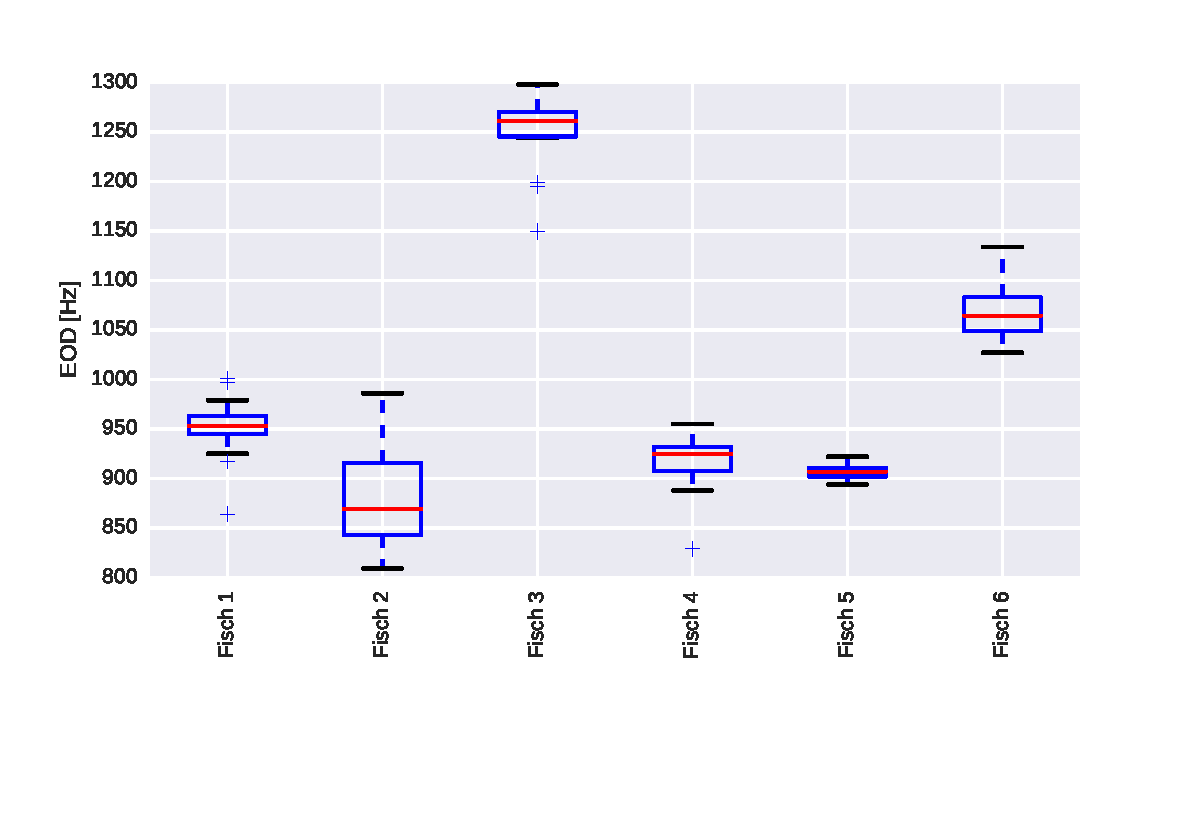
\includegraphics[height=8.5cm]{Abbildungen/eod_boxplot}
\caption{\label{fig:eods}Graphik zeigt die EOD Verteilung der Fische �ber den gesamten Versuchszeitraum inklusive Vorversuche.}
\end{figure}

Der EOD Median von Fisch 1 (siehe Abbildung \ref{fig:eods}) liegt dabei bei 953 Millivolt. Der Median von Fisch 2 hingegen liegt etwas tiefer und zwar bei 869 Millivolt. Fisch 3 hatte von allen Versuchstieren die h�chste EOD Frequenz und lag bei einem Median von 1261 Millivolt. Der Median von Fisch 4 befand sich bei 925 Millivolt und der von Fisch 5 bei 907 Millivolt. Fisch 6 besa� mit einem Median von 1064.5 Millivolt die zweit h�chste EOD Frequenz.


\begin{figure}[ht]
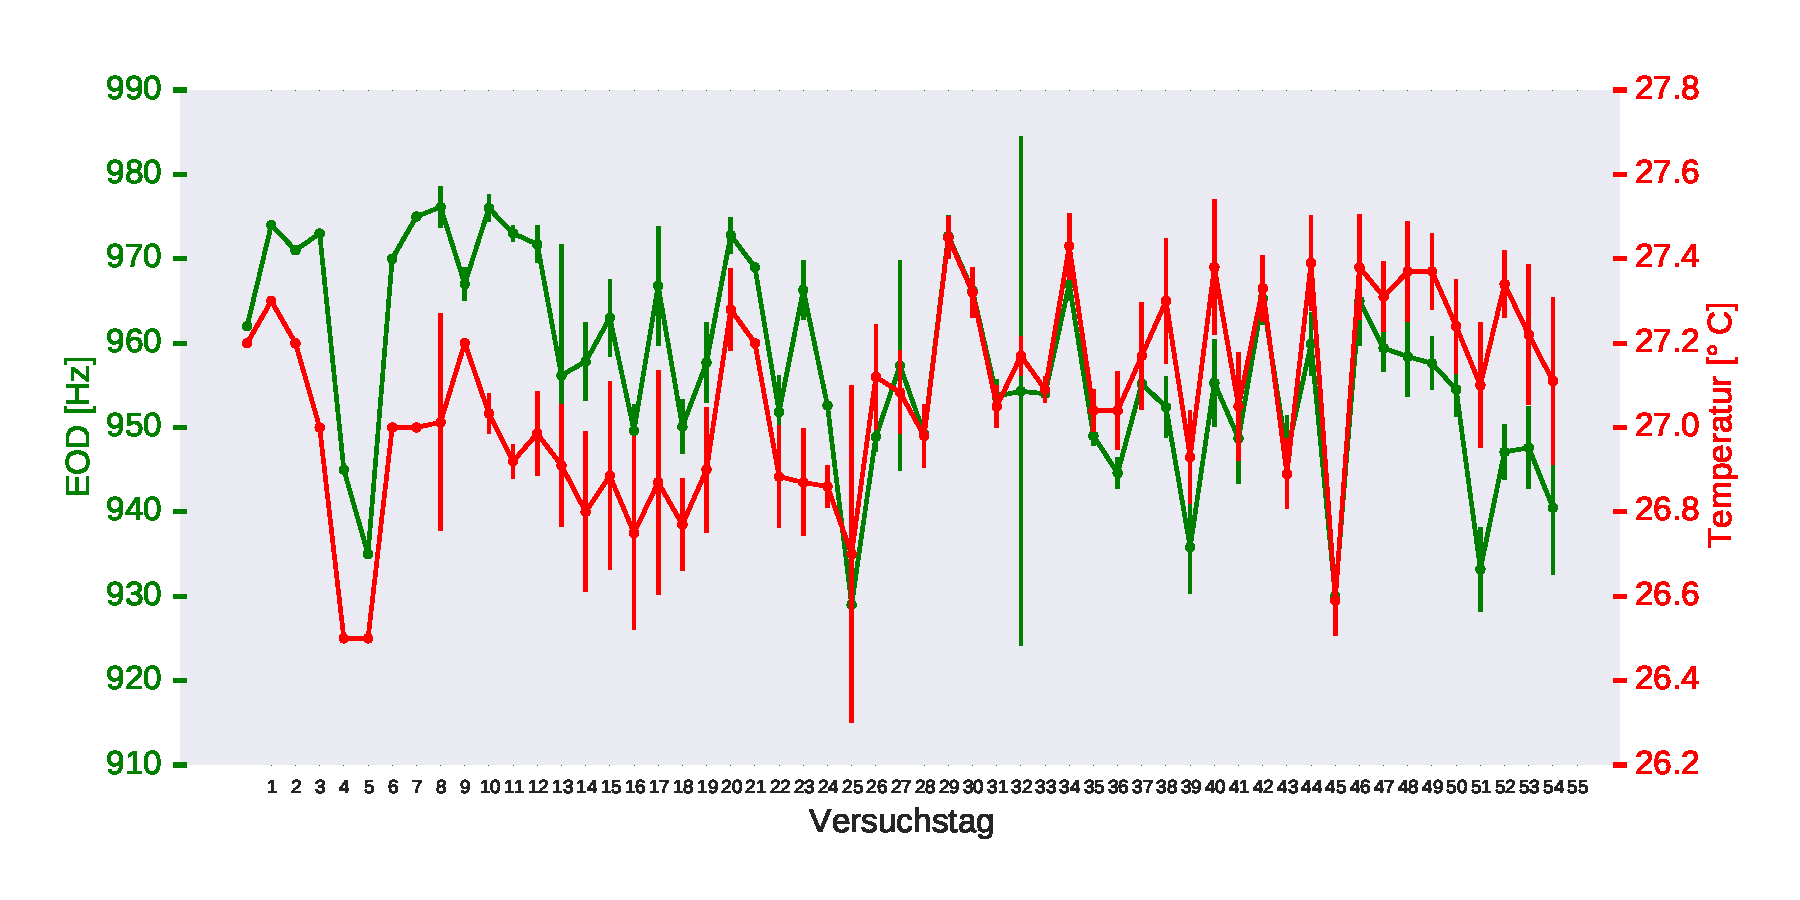
\includegraphics[height=6.5cm]{Abbildungen/date_temperature_eod_plot2015albi02}
\caption{\label{fig:temperatureod1}Die Graphik zeigt die Wassertemperaturen (rote Kurve) und die EOD Frequenzen von Fisch 1 in gr�n �ber die gesamte Versuchszeit einschlie�lich Vorversuche.}
\end{figure}

\begin{figure}[ht]
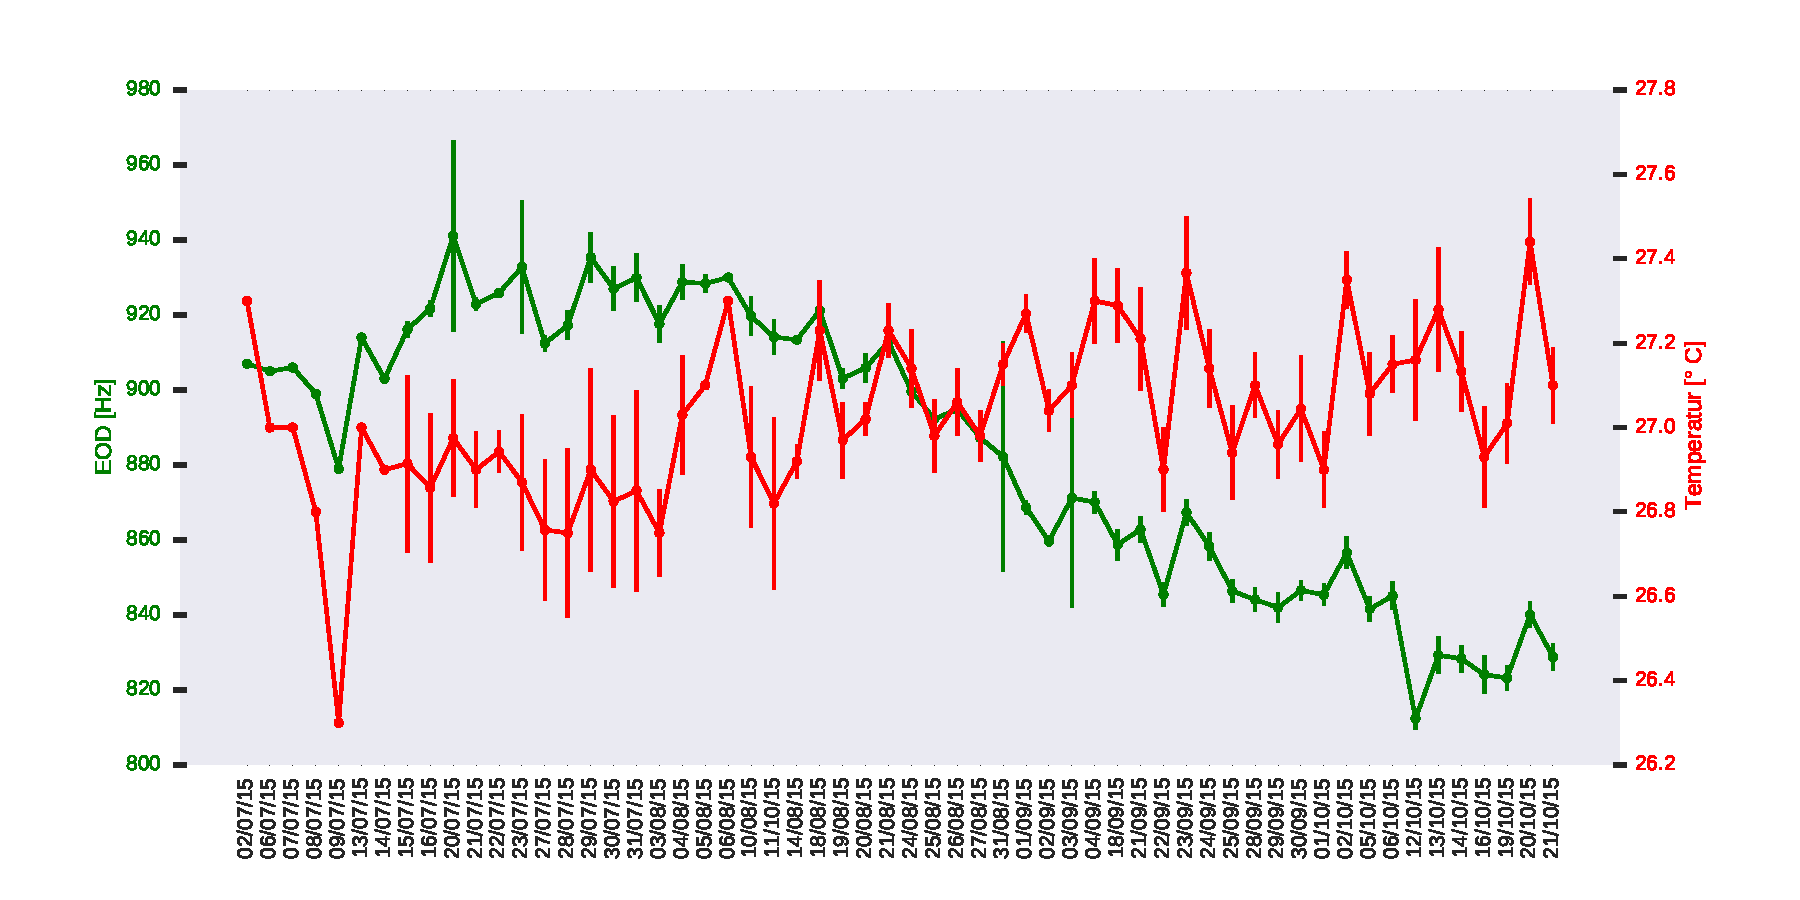
\includegraphics[height=6.5cm]{Abbildungen/date_temperature_eod_plot2015albi01}
\caption{\label{fig:temperatureod2}Die Graphik zeigt die Wassertemperaturen (rote Kurve) und die EOD Frequenzen von Fisch 2 in gr�n �ber die gesamte Versuchszeit einschlie�lich Vorversuche.}
\end{figure}


\begin{figure}[ht]
\subfigure[Fisch 3]
{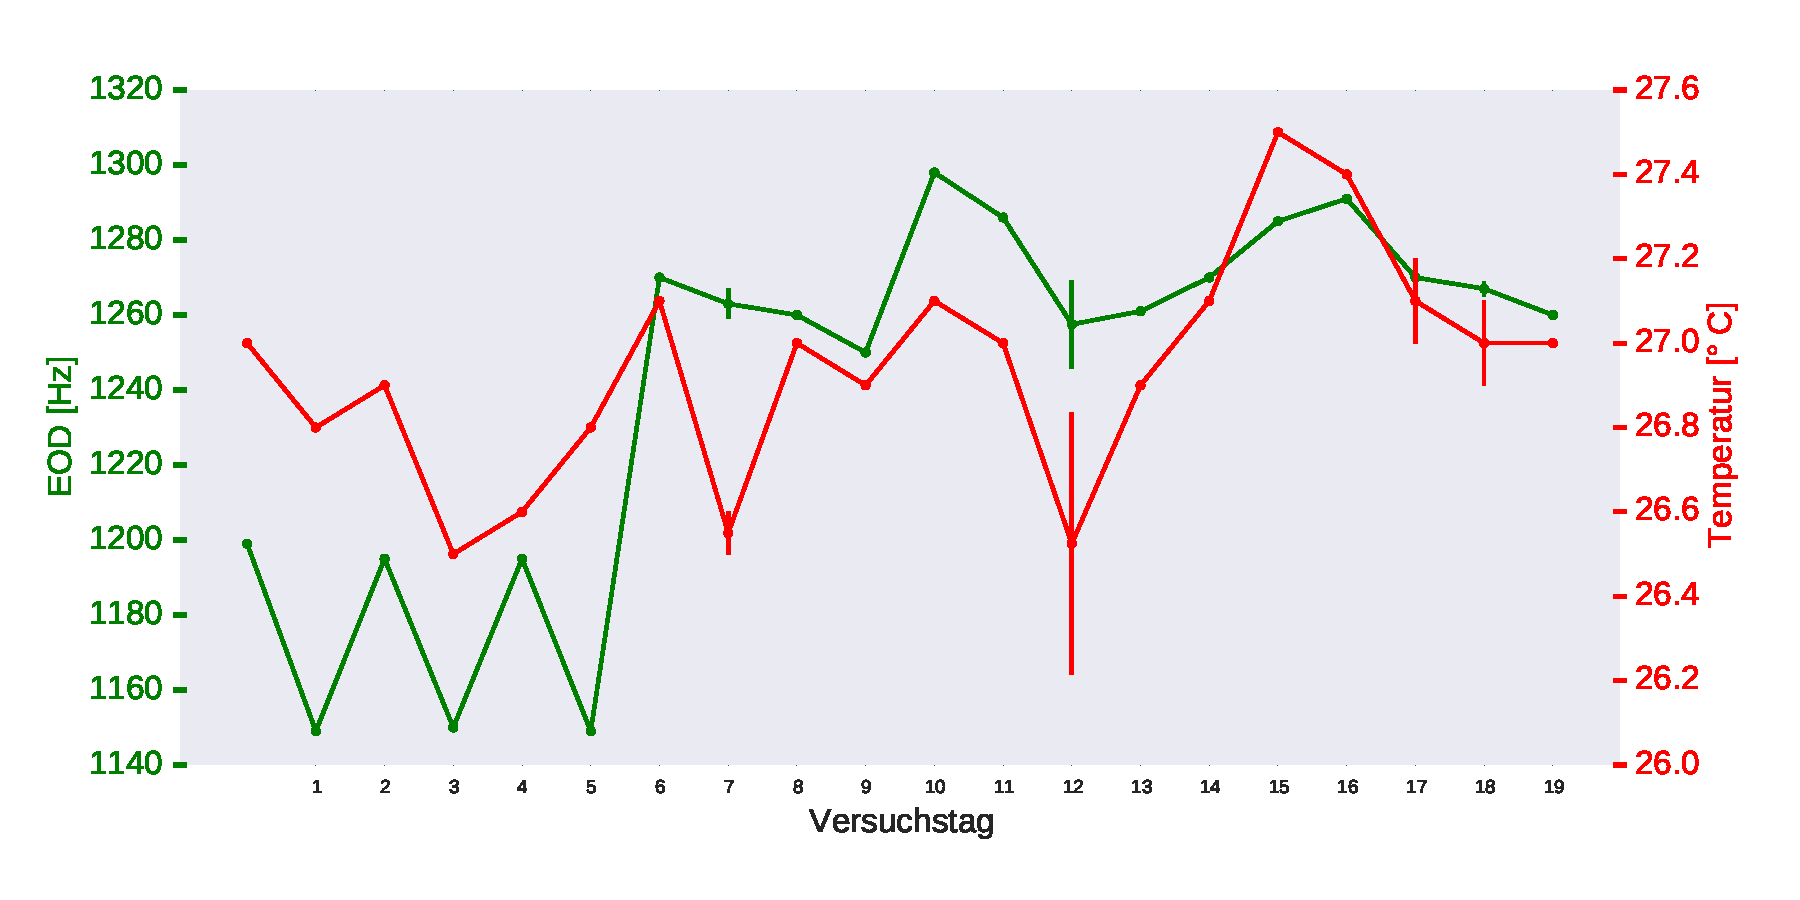
\includegraphics[height=4cm]{Abbildungen/date_temperature_eod_plot2014albi08}}
\subfigure[Fisch 4]
{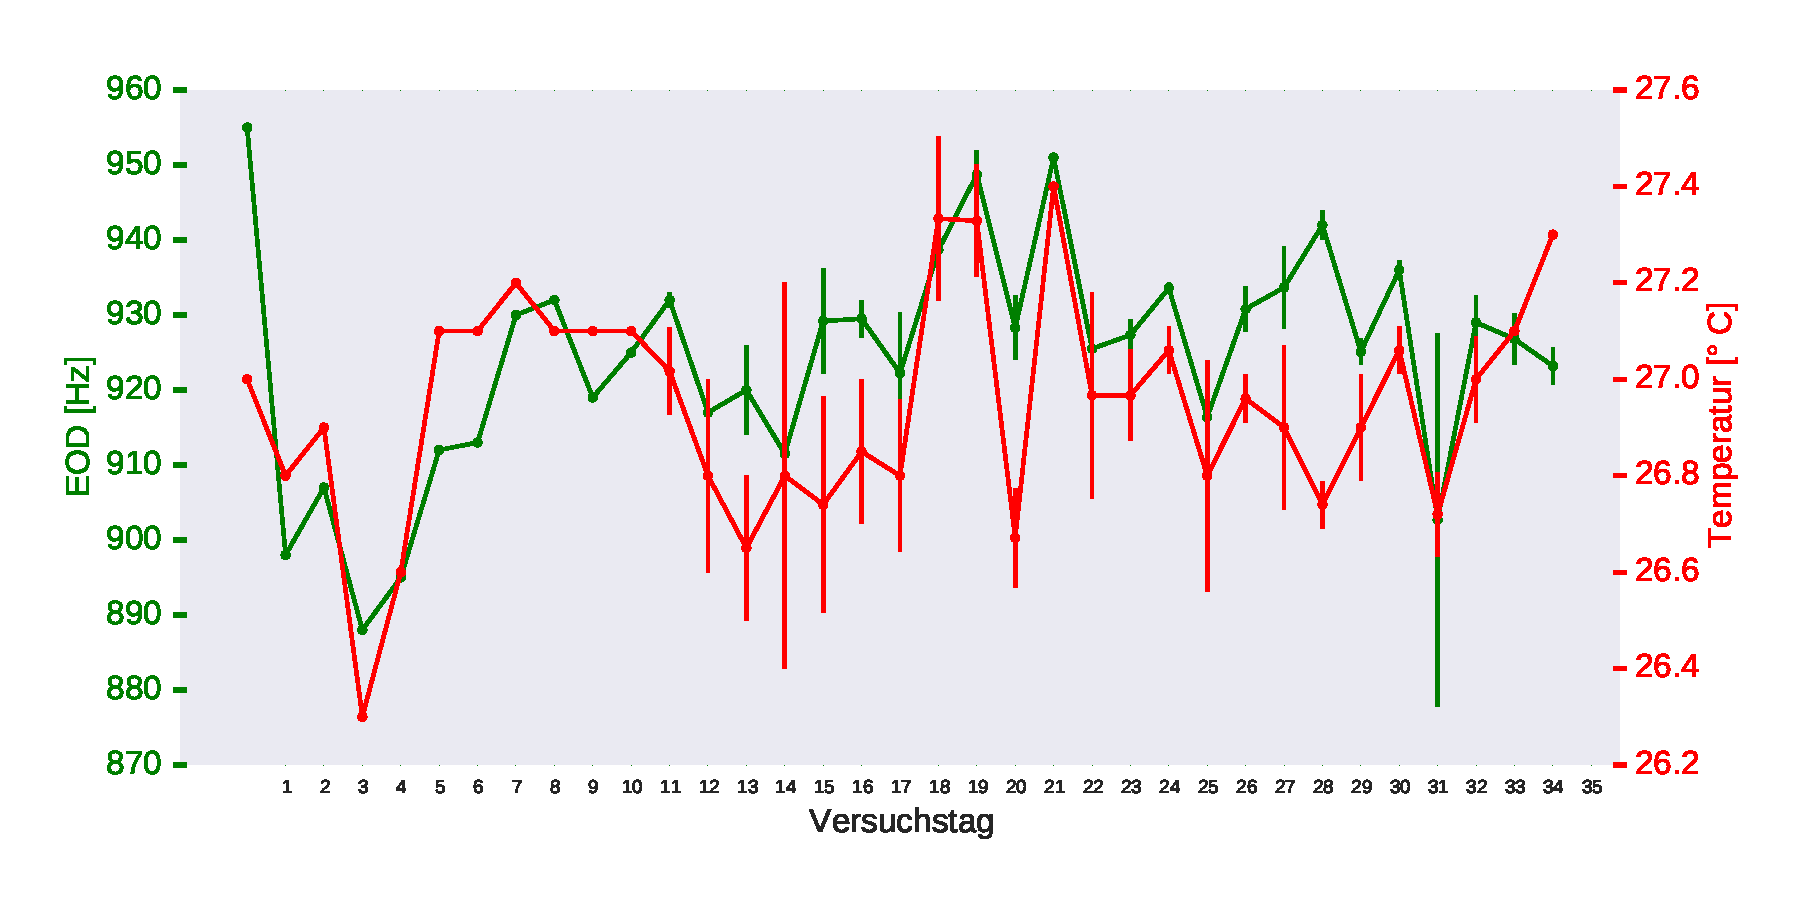
\includegraphics[height=4cm]{Abbildungen/date_temperature_eod_plot2013albi14}}
\subfigure[Fisch 5]
{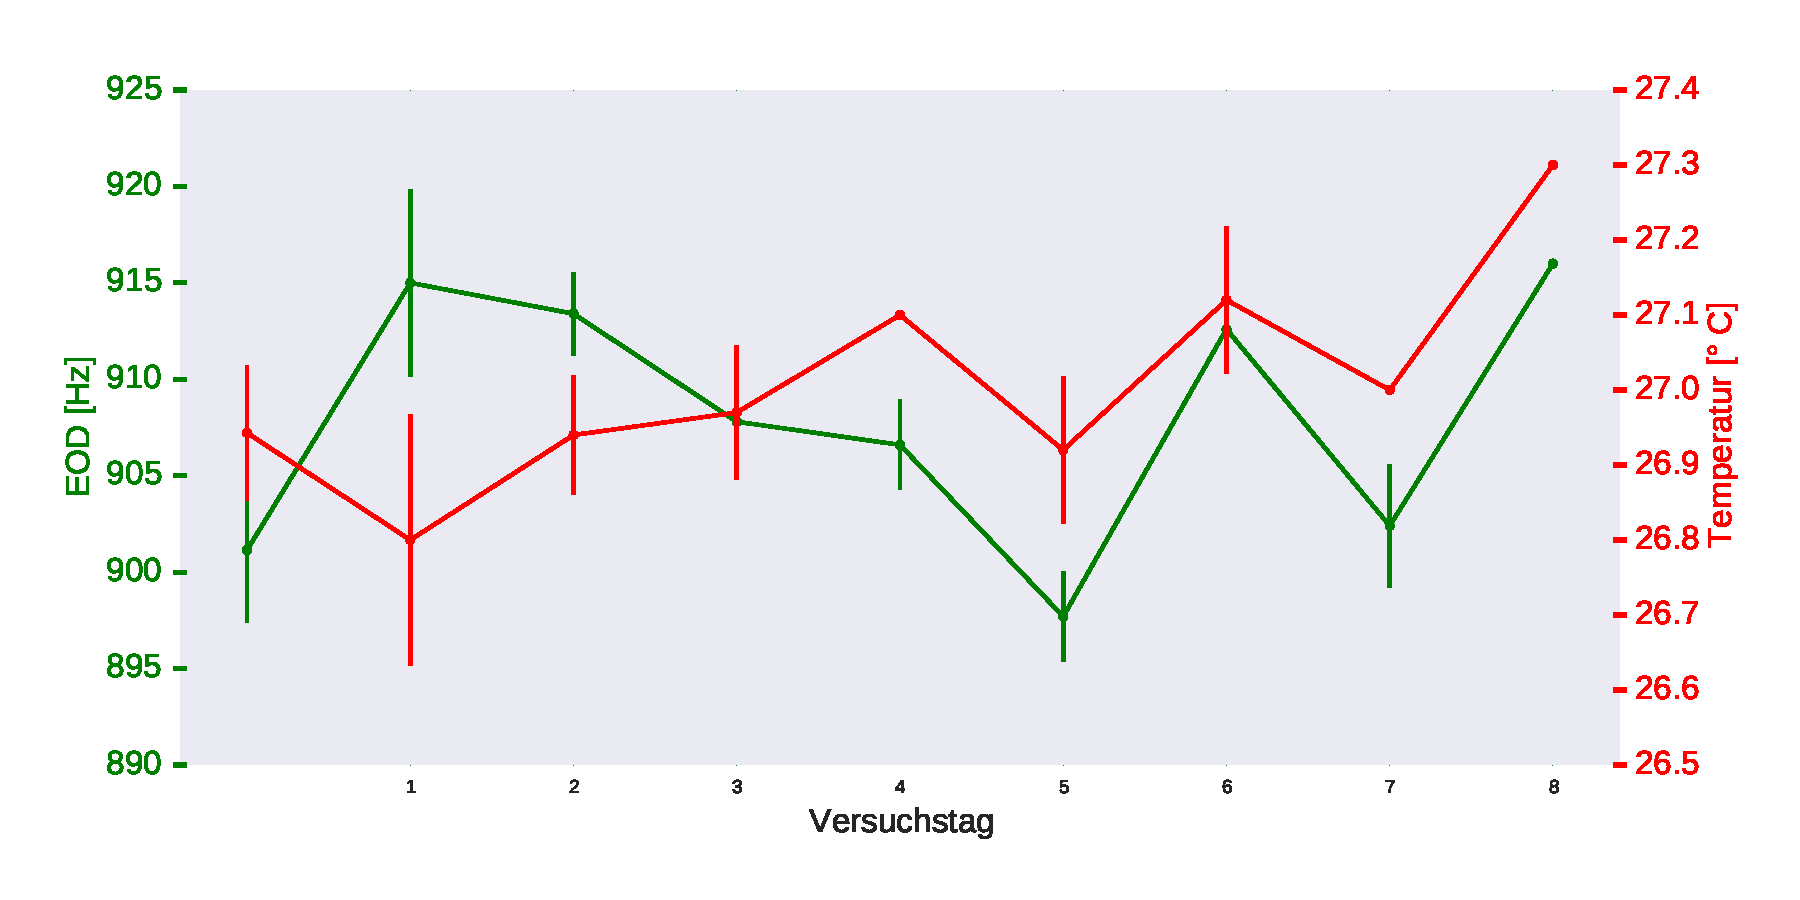
\includegraphics[height=4cm]{Abbildungen/date_temperature_eod_plot2013albi09}}
\subfigure[Fisch 6]
{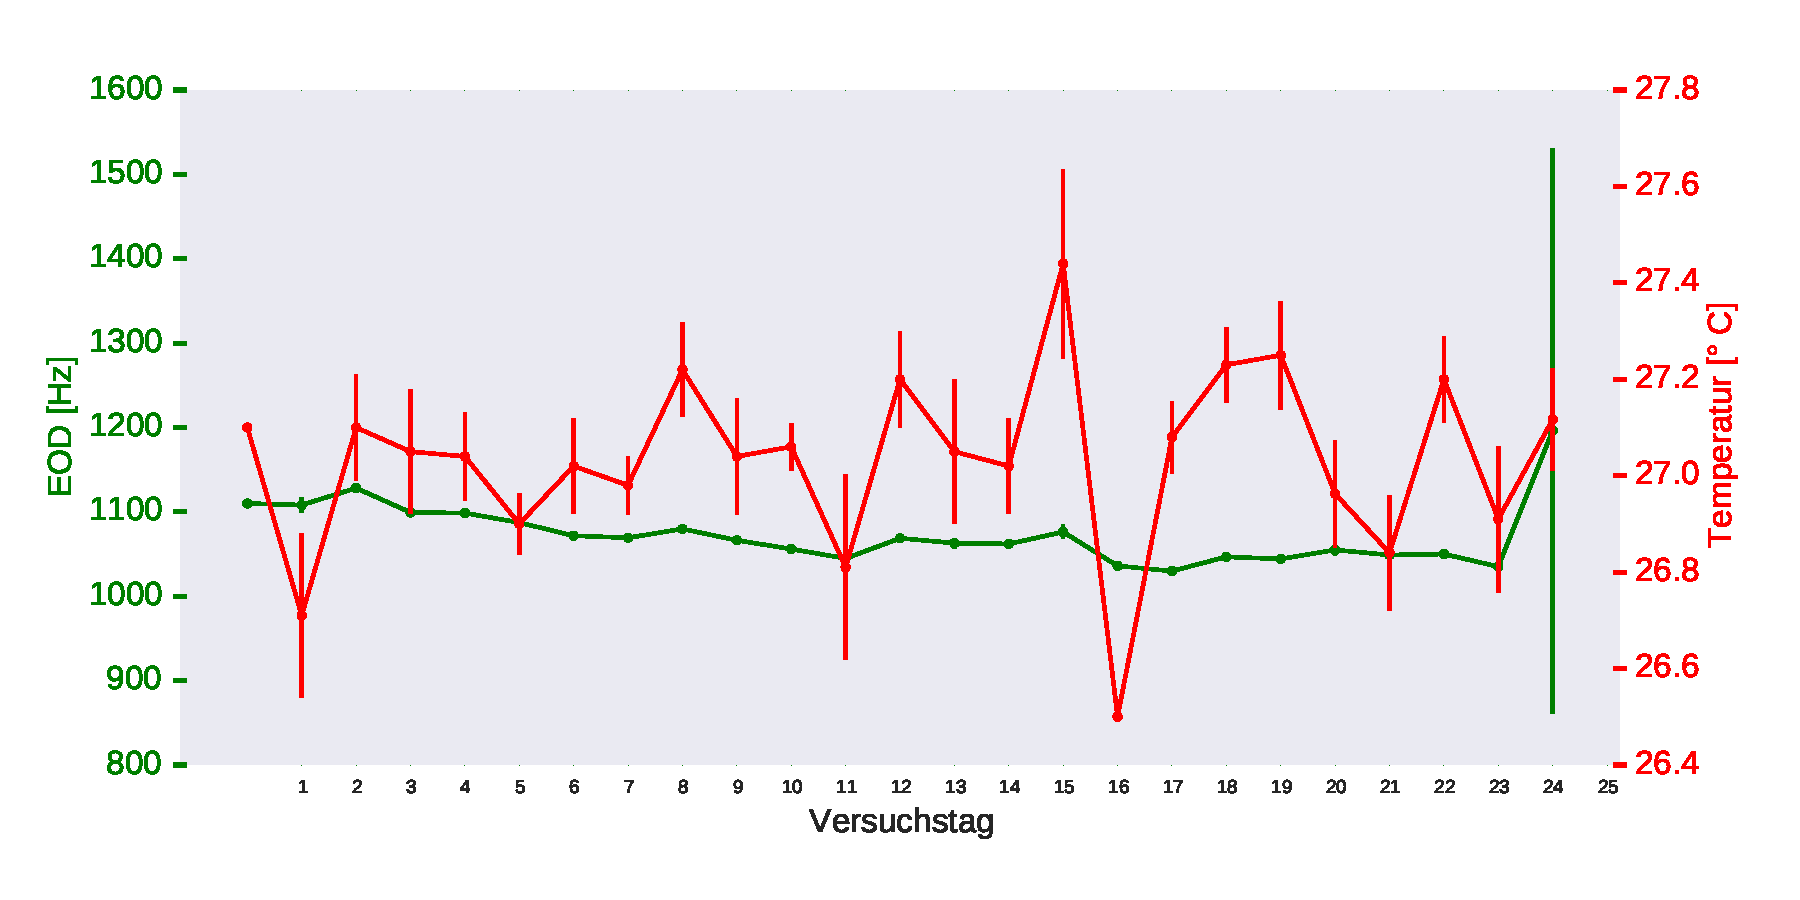
\includegraphics[height=4cm]{Abbildungen/date_temperature_eod_plot2012albi01}}
\caption{\label{fig: temperatureod3}  Wassertemperaturen (rote Kurve) und die EOD Frequenzen von Fisch 3, 4, 5, 6 in gr�n �ber die gesamte Versuchszeit einschlie�lich Vorversuche.}
\end{figure}


\begin{figure}[ht]
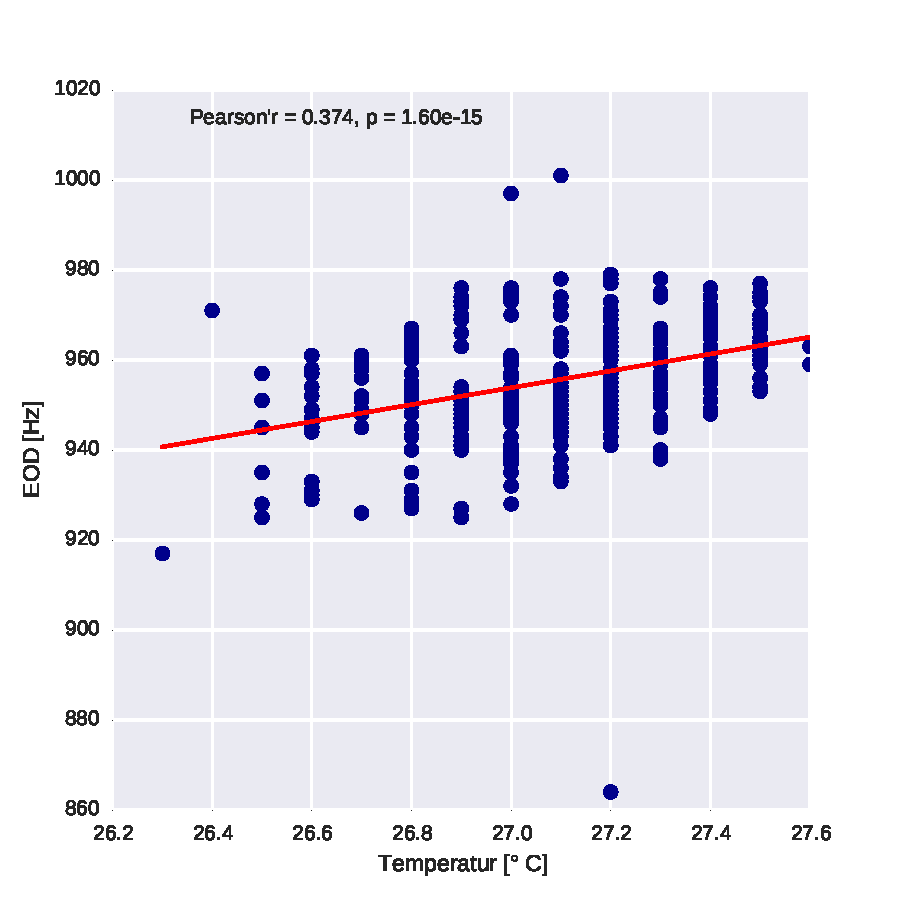
\includegraphics[height=8.5cm]{Abbildungen/regression1}
\caption{\label{fig:regression1}Regressionsgerade von Temperatur und EOD Fisch 1.}
\end{figure}


\begin{figure}[ht]
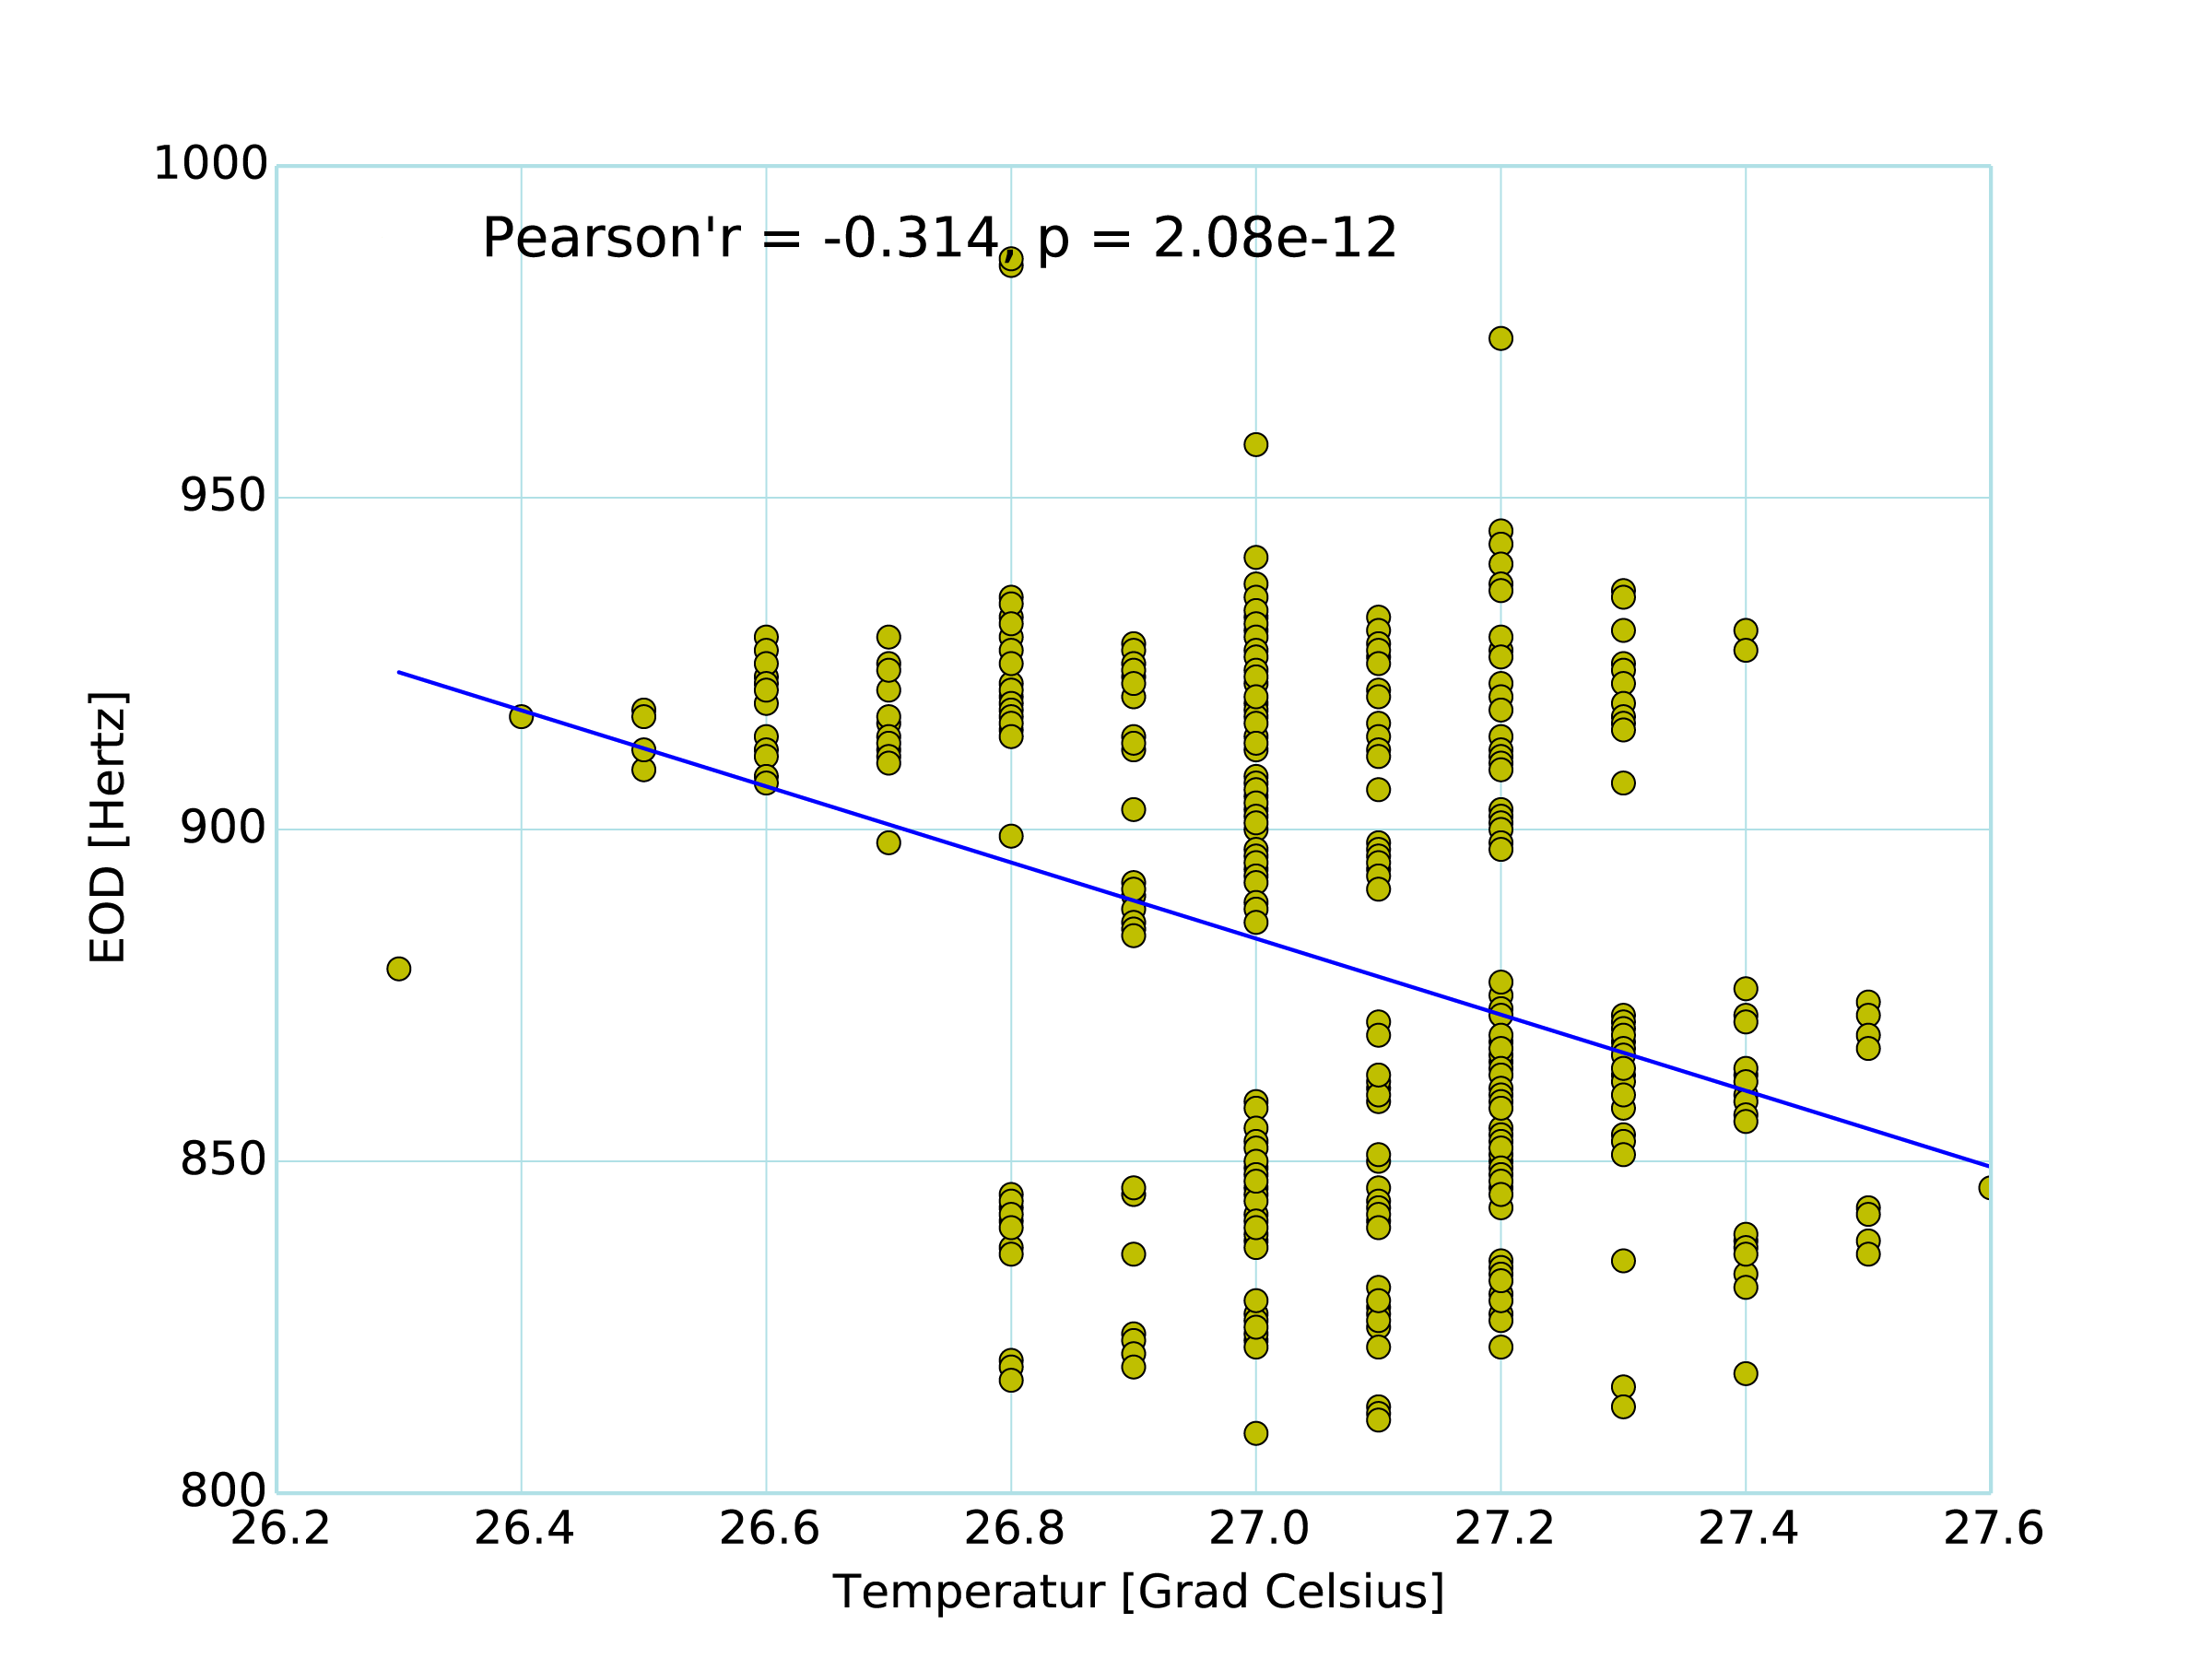
\includegraphics[height=8.5cm]{Abbildungen/regression2}
\caption{\label{fig:regression2}Regressionsgerade von Temperatur und EOD Fisch 2.}
\end{figure}



\section{Vorversuche}
\subsection{Eingew�hnung}

Fish 1 und Fisch 2 gingen nach 9 Versuchstagen in die n�chste Phase die "Konditionierung auf den gew�nschten Reiz" �ber. Da Fisch 3 und Fisch 4 schlechter kooperierten, ginge diese erst nach elf Versuchstagen in die n�chste Phase �ber.


Paper Konditionierung?

